% begin module rational-functions
\begin{frame}
\frametitle{Rational Functions}
\begin{definition}[Rational Function]
A rational function is a quotient of two polynomials; that is, a function of the form
\[
f(x) = \frac{g(x)}{h(x)},
\]
where $g$ and $h$ are polynomials.
\end{definition}
\begin{columns}[c]
\column{.4\textwidth}
\uncover<2->{
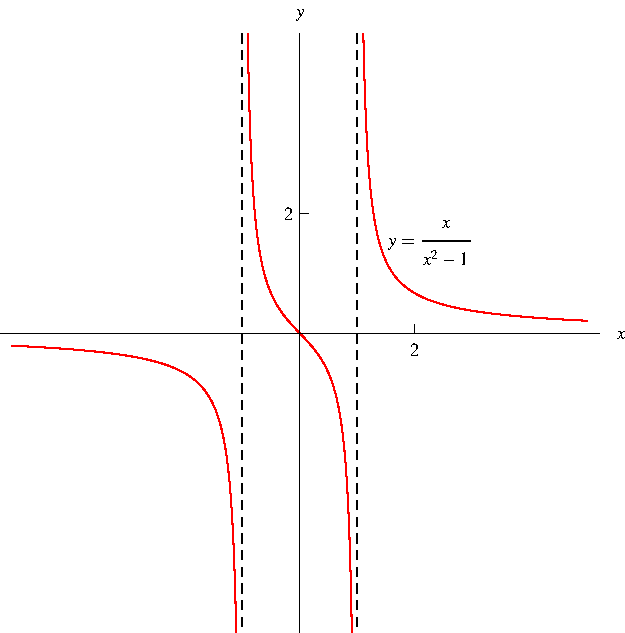
\includegraphics[height=4cm]{precalculus/pictures/01-02-rational.pdf}%
}
\column{.6\textwidth}
\uncover<2->{
\begin{example}[$x/(x^2-1)$]
The function
\[
f(x) = \frac{x}{x^2-1}
\]
is a rational function.
\end{example}
}
\end{columns}
\end{frame}
% end module rational-functions
